%!TEX root = ../../thesis.tex

\section{Related Work}
\label{sec:coqa-rw}

Conversational question answering is directly related to \tf{dialogue}. Building conversational agents, or dialogue systems to converse with humans in natural language is one of the major goals of natural language understanding. The two most common classes of dialogue systems are: \ti{task-oriented}, and \ti{chit-chat} (or \ti{chatbot}) dialogue agents.  Task-oriented dialogue systems are designed for a particular task and set up to have short conversations (e.g., booking a flight or making a restaurant reservation). They are evaluated based on task-completion rate or time to task completion. In contrast, chit-chat dialogue systems are designed for extended, casual conversations, without a specific goal. Usually, the longer the user engagement and interaction, the better these systems are.

Answering questions is also a core task of dialogue systems, because one of the most common needs for humans to interact with dialogue agents is to seek information and ask questions of various topics. QA-based dialogue techniques have been developed extensively in automated personal assistant systems such as Amazon's \sys{Alexa}, Apple's \sys{Siri} or \sys{Google Assistant}, either based on structured knowledge bases, or unstructured text collections. Modern dialogue systems are mostly built on top of deep neural networks. For a comprehensive survey of neural approaches to different types of dialogue systems, we refer readers to \cite{gao2018neural}.

\begin{figure}[!t]
    \center
    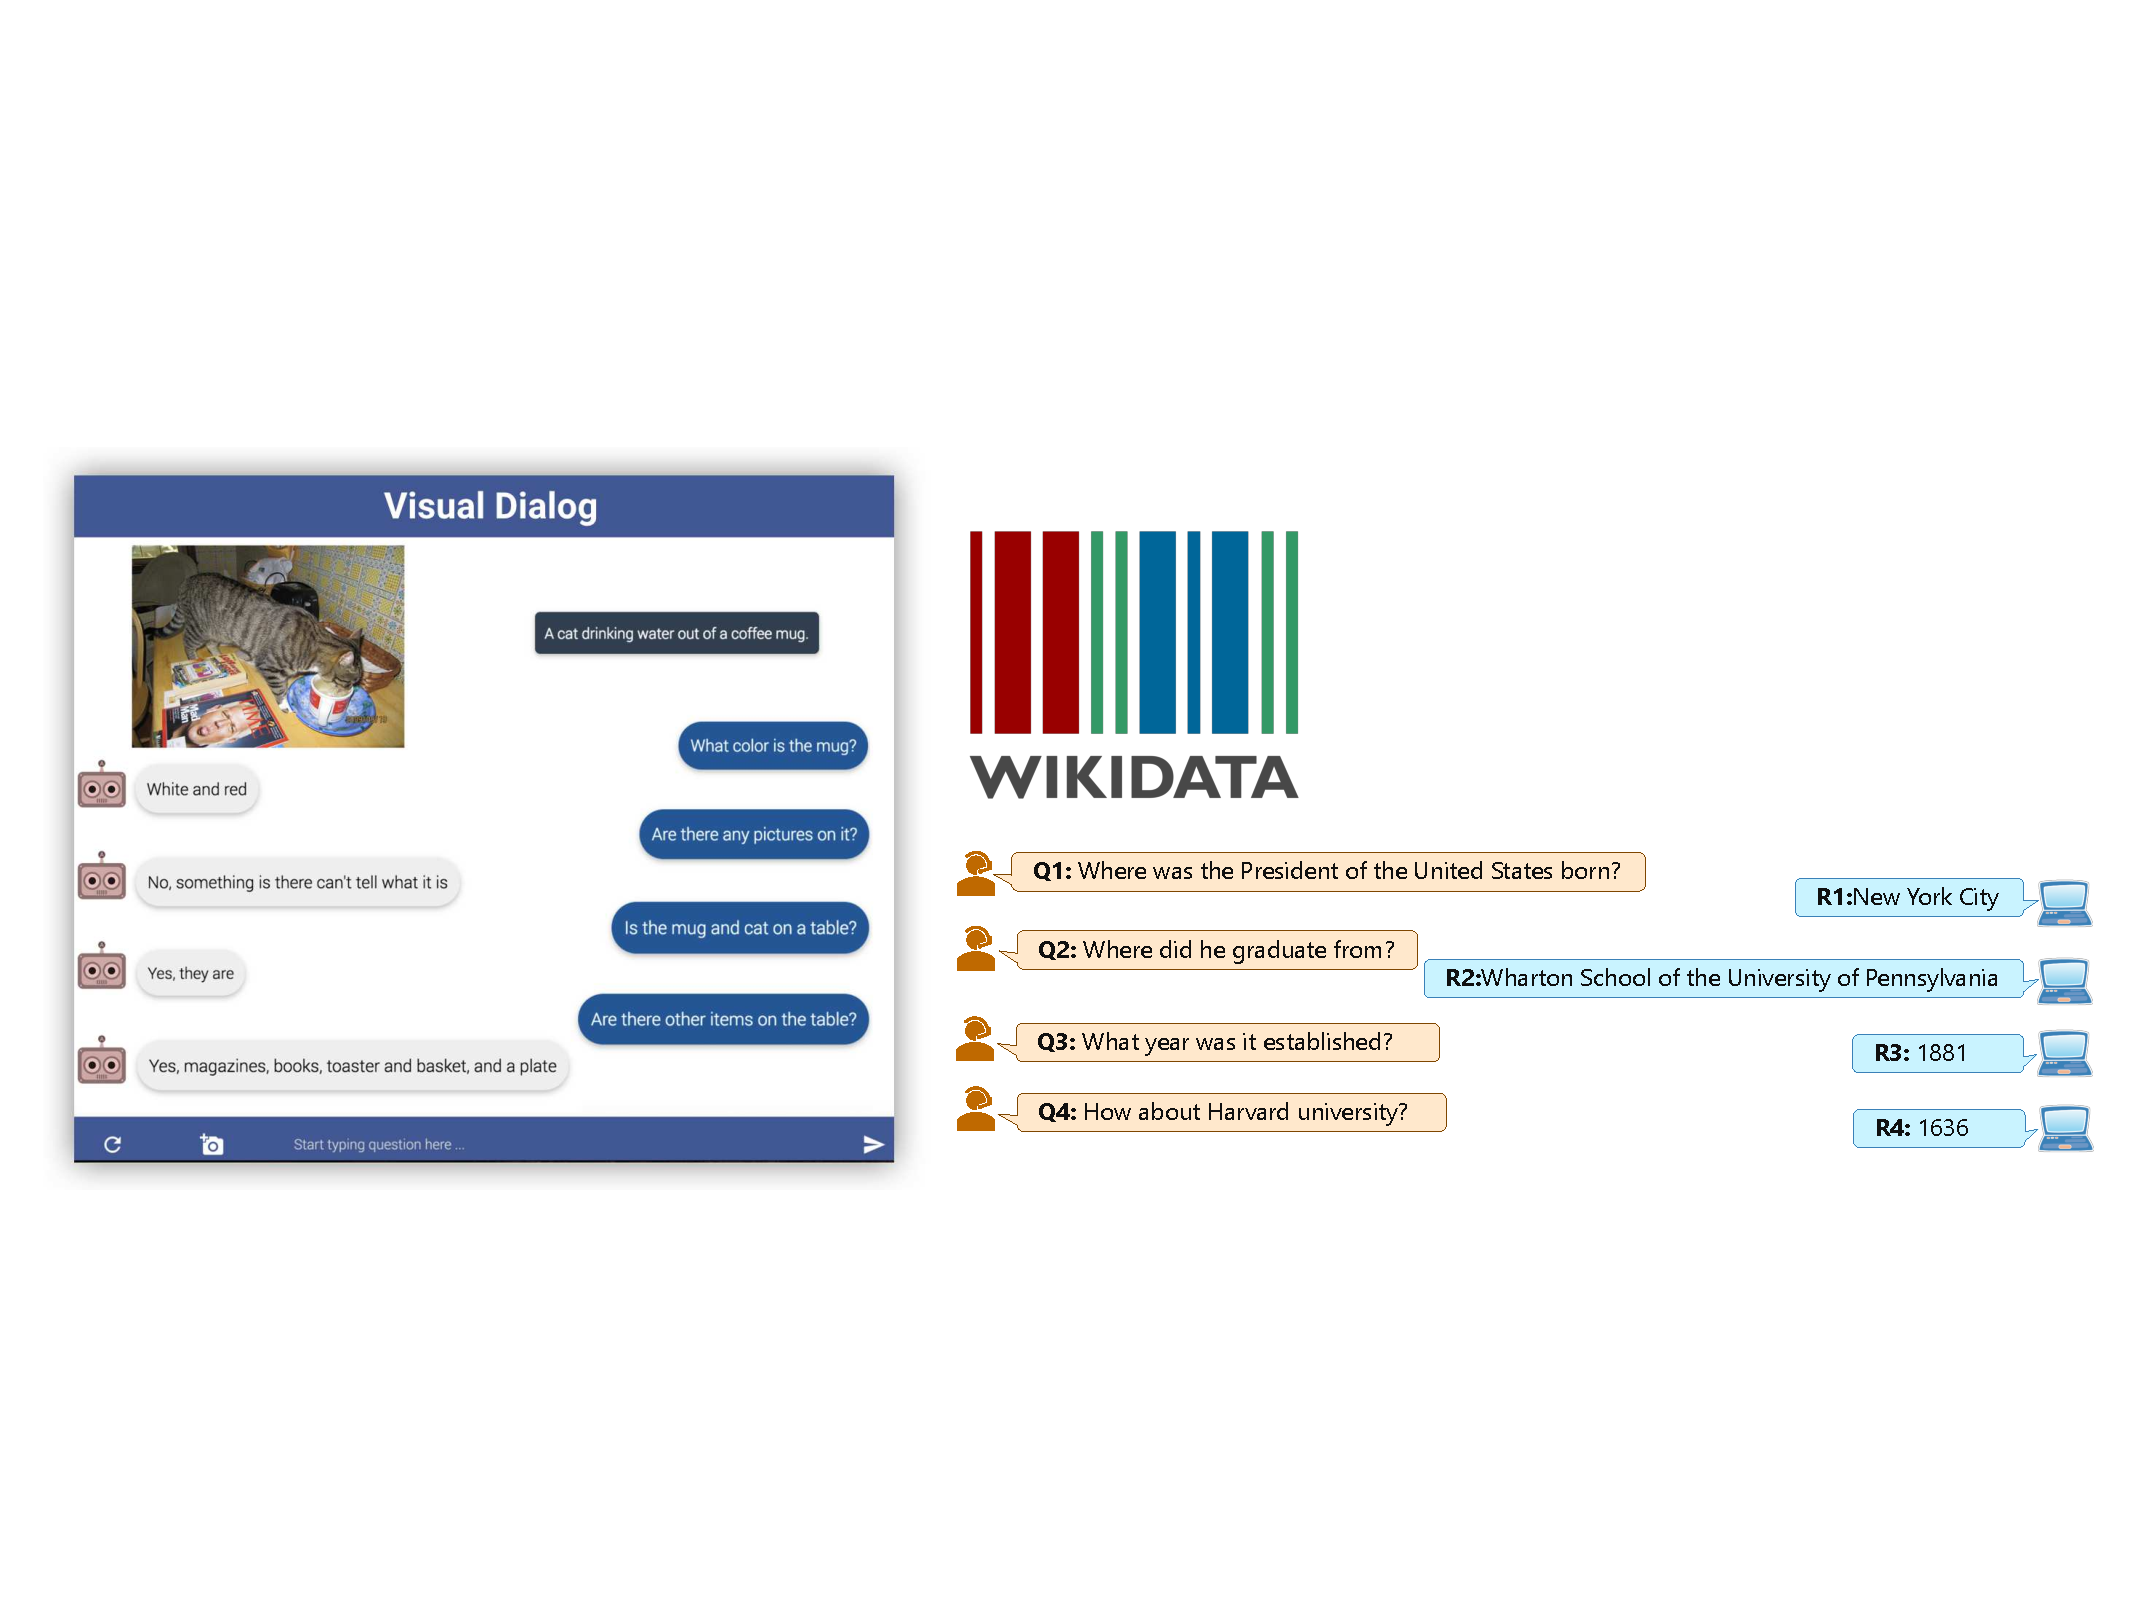
\includegraphics[scale=0.45]{img/other_coqa_tasks.pdf}
    \longcaption{Other conversational question answering tasks on images and KBs}{\label{fig:other-coqa-tasks}Other conversational question answering tasks on images (left) and KBs (right). Images courtesy: \cite{das2017visual} and \cite{guo2018dialog} with modifications.}
\end{figure}

Our work is closely related to the \ti{Visual Dialog} task of \cite{das2017visual} and the \ti{Complex Sequential Question Answering} task of \cite{saha2018complex}, which perform conversational question answering on images and a knowledge graph (e.g. \sys{WikiData}) respectively, with the latter focusing on questions obtained by paraphrasing templates. Figure~\ref{fig:other-coqa-tasks} demonstrates an example from each task. We focus on conversations over a passage of text, which requires the ability of reading comprehension.

Another related line of research is \ti{sequential question answering}~\cite{iyyer2017search,talmor2018web}, in which a complex question is decomposed into a sequence of simpler questions. For example, a question \ti{What super hero from Earth appeared most recently?} can be decomposed into the following three questions: 1) \ti{Who are all of the super heroes?}, 2) \ti{Which of them come from Earth?}, and 3) \ti{Of those, who appeared most recently?}. Therefore, their focus is how to answer a complex question via sequential question answering, while we are more interested in a natural conversation of a variety of topics while the questions can be dependent on the dialogue history.
